
\chapter{Distributional RL}
\label{sec:distr_rl}


\section{Distributional RL}

Recent research has been done demonstrating the importance of learning the value
distribution,
i.e, the distribution of the random return received by a RL agent.
This differs from the common RL approach which is focused on learning the expected value
 of this return.

One of the major goals of RL is to teach an agent so that it learns how to act so that it
maximizes its expected utility, Q \cite{Sutton1998}
Bellman's equation describes this value Q in terms of the expected reward and expected
outcome of the 
random transition $(x,a) \to (X',A')$, showing the
particular recursive relationship between the value of a state and the values of its
successor states:
\begin{equation}
    Q(x,a) = \mathbb E[R(x,a)] + \gamma \mathbb E[Q(X',A')] \label{eq:bellman}
\end{equation}

Distributional RL aims to go beyond the notion of \textit{value} and training to study
instead the random 
return Z.

\subsection{Example showing interest in learning the distribution}

Imagine the example in which we are playing a board game and we roll 2 dices.
If we get a 3, we fall in prison and need to pay 2000CHF (ie reward of -2000CHF), whereas
 otherwise we 
we collect a salary of 200CHF (ie reward of +200CHF).
If we consider the common reinforcement learning approach and we compute the expected
immediate ($\gamma = 1$)
reward: 

\begin{equation}
    \mathbb E[R(x)]= \frac{1}{36} (\SI{-2000}{\CHF}) + \frac{35}{36} (\SI{+200}{\CHF}) = \SI{138.88}{\CHF} 
\end{equation}

Hence, the expected immediate return is +138.88CHF. However, in any case we will get a
return of +138.88CHF.
Instead:

$R(x) = \begin{cases}  \SI{-2000}{\CHF} , & \mbox{w.p } \frac{1}{36} \\ \mbox{ }\SI{+200}{\CHF}, & \mbox{w.p } \frac{35}{36} \end{cases}$
\newpage
We define the random return $Z^\pi(x,a)$ as the random variable that represents the sum
of discounted rewards
obtained by 
starting from position \textit{x} taking action \textit{a} and thereupon following
policy $\pi$.

This variable captures intrinsic randomness from:
\begin{enumerate}
    \item Immediate rewards
    \item Stochastic dynamics
    \item Possibly an stochastic policy
\end{enumerate}

Having defined $Z^\pi(x,a)$, we can clearly see that:
\begin{equation}
    Q^\pi(x,a) = \mathbb E[Z^\pi(x,a)]
\end{equation}

Z is also described by a recursive equation, but of a distributional nature:
\begin{eqnarray}
    Z^\pi(x,a) \stackrel{D}{=} R(x,a) + \gamma Z(x',a') \label{eq:distrbellman}
\end{eqnarray}
where $x'\backsim\ p(\cdot|x,a) \text{ and } a' \backsim\ \pi(\cdot |x')$

where $\stackrel{D}{=}$ denotes that the RV on both sides of the equation share the same
 probability distribution.
The \textit{distributional Bellman equation} defined in \eqref{eq:distrbellman}, states
that the distribution of 
Z is characterized by the interaction of 3 RV's: the random variable reward R, the next
state-action (X',A')
and its random return 
Z(X',A'). From here on, we will view $Z^\pi$ as a mapping from state-action pairs to
distributions over
returns, and we call this distribution the \textit{value distribution}.

\subsection{Distributional Bellman Operator}

In the policy evaluation setting \cite{Sutton1998}, one aims to find the value function
$V\pi$ associated
with a given fixed policy $\pi$. In the distributional case, we aim to find $Z\pi$.
\cite{Bellemare2017} defined the Distributional Bellman operator $T^\pi$.
We view the reward function as a random vector R $\in \mathbb{Z}$ and define the transition
operator 
$P^\pi: \mathbb{Z} $ \ra $\mathbb{Z}$
\begin{eqnarray}
    P^\pi Z(x,a) \stackrel{D}{=} Z(X',A')\\
    X'\backsim\ P(\cdot|x,a) \text{ and } A' \backsim\ \pi(\cdot |X')
\end{eqnarray}
where we use capital letters to emphasize the random nature of the next state-action pair
 (X',A')
Then, the Distributional Bellman operator $T^\pi$ is defined as:
\begin{eqnarray}
    T^\pi Z(x,a) \stackrel{D}{=} R(x,a) + \gamma P^\pi Z(x,a) \label{eq:distrbellmanoperator}
\end{eqnarray}


\cite{Bellemare2017} showed that \eqref{eq:distrbellmanoperator} is a contraction
mapping in Wasserstein metric whose unique fixed point is the 
random return $Z^\pi$.

\subsubsection{Wasserstein metric:}

The p-Wasserstein metric $W_p$, for $p \in [1,\infty]$, also known as the Earth Mover's 
Distance when $p=1$ is an integral probability metric between distributions. The
p-Wasserstein distance is characterized 
as the $L^p $ metric on inverse cumulative distribution functions (CDF). Tht is, the
p-Wasserstein metric
between distributions $U $ and $Y $ is given by:
\begin{equation}
    W_p(U,Y) = \big (  \int_{0}^{1} | F_Y^{-1}(w) - F_U^{-1}(w) |^p dw   \big )^{\frac{1}{p}}
\end{equation}

where for a random variable Y, the inverse CDF $F_Y^{-1}$ of Y is defined by:
\begin{equation}
    F_Y^{-1}(w) \coloneqq \text{inf} \big\{ y \in \mathbb{R} \; | w \; \leq   F_Y(w)    \big\}
\end{equation}
where $F_Y(w) = Pr(y \leq Y)$. \\
\todo{Add Figure 2.1 in \cite{Dabney2018}}
Unlike the Kullback-Leibler divergence , the Wasserstein metric is a true probability
metric and considers both the probability of
and the distance between various outcome events, which makes it well-suited to domains 
where an underlying similarity in outcome is more important than exactly matching likelihoods.

\subsubsection{Contraction in $\hat{d}_p$:}

Let $\mathcal{Z}$  be the space of action-value distributions:
\begin{eqnarray}
    \mathcal{Z} = \big \{ Z \;| \; \mathcal{X} \times  \mathcal{A} \ra \wp (\mathbb{R} )\\
    \mathbb{E} [ | Z(x,a)|^p < \infty, \forall (x,a), p\geq 1        ]\big \}
\end{eqnarray}
\todo{check first line the $\wp$}

Then, for two action-value distribution $Z_1, Z_2 \in \mathcal{Z}$, the maximal form of the 
Wasserstein metric is defined by:
\begin{equation}
    \hat{d}_p(Z_1,Z_2) \coloneqq \underset{x,a} {\text{sup}}  \;W_p(Z_1(x,a),Z_2(x,a))
\end{equation}

\cite{Bellemare2017} showed that $\hat{d}_p$ is a metric over value distributions
and furthermore, the distributional
Bellman operator $T^\pi$ is a contraction in $\hat{d}_p$.
Consider the process $Z_{k+1} \coloneqq T^\pi Z_{k}$, starting with some $Z_{0} \in \mathcal{Z}$. \\
$T^\pi Z: \mathcal{Z} $ \ra $\mathcal{Z}$ is a $\gamma$-contraction in the Wasserstein
metric $\hat{d}_p$, which implies that 
not only the first moment (expectation) converges exponentially to $ Q^\pi$, but also in
 all moments.\newline
\textbf{Lemma 1:} (Lemma 3 in \cite{Bellemare2017} )\\
$T^\pi$ is a $\gamma$-contraction: for any two $Z_1, Z_2 \in \mathcal{Z}$,
\begin{equation}
    \hat{d}_p(T^\pi Z_1, T^\pi Z_2) \leq \gamma \hat{d}_p(Z_1,Z_2)
\end{equation}
Using Banach's fixed point theorem, it is proven that $T^\pi$ has a unique fixed point,
which by inspection must be $Z^\pi$.

Hence the $\hat{d}_p$ metric is shown to be useful metric for studying behavior of
distributional RL algorithms, and to showed their convergence to a fixed point.
Moreover, shows than en effective way to learn a value distribution is to attempt minimize
the Wasserstein distance between a distribution Z and its distributional Bellman update
$T^\pi Z$, analogously to the way that TD-learning attempts to iteratively minimize
the $L^2$ distance between Q and $TQ$.

We have so fare considered a policy evaluation setting, ie trying to learn a value
distribution for a fixed policy $\pi $, and we studied
the behavior of its associated distributional operator $T^\pi $.
In the control setting, ie, when we try to find a policy $\pi^{*} $ that maximizes a
value, or its distributional analogous, ie that
induces an optimal value distribution. However, while all optimal policies attain the
same value $Q^{*}$, in general there are
many optimal value distributions.

The distributional analogue of the Bellman optimality operator converges, in a weak sense,
to the set of optimal value distributions, but
this operator is \textit{not a contraction in any metric between distributions.}.\\
Let $\Pi^*$ be the set of optimal policies.\\
\textbf{Definition 1:} 
An optimal value distribution is the value distribution of an optimal policy. The set of optimal value distributions is 
\begin{equation*}
    \mathcal{Z^*} \coloneqq \big\{ Z^{\pi^*} | \pi^{*} \in  \Pi^*   \big\}
\end{equation*}
Not all value distributions with expectation $Q^*$ are optimal, but they must match the full distribution of the return
under some optimal policy.
\textbf{Definition 2:} 
A greedy policy $\pi$ for Z $in \mathcal{Z}$ maximizes the expectation of Z. The set of greedy policies for Z is:
\begin{equation*}
    \mathcal{G_Z} \coloneqq \big\{ \pi  \; | \sum_a \pi(a|x) \mathbb E (Z(x,a) = \underset{a'\in \mathcal{A}}{\text{max}}  \; Q(x',a')   \big\}
\end{equation*}

We will call a \textit{distributional Bellman optimality operator} any operator $\mathcal{T}$ which implements a greedy selection
rule, ie:
\begin{equation*}
    \mathcal{T}Z = \big\{ \mathcal{T}^\pi Z \; \text{for some}\; \pi \in   \mathcal{G_Z} \big\}
\end{equation*}
As in the policy evaluation setting, we are interested in the behavior of the iterates 
$Z_{k+1} := \mathcal{T}Z_k, Z_0 \in \mathcal{Z}$.
Lemma 4 in \cite{Bellemare2017} shows that $\mathbb E Z_k$ behaves as expected:
\textbf{Lemma 4:} Let $Z_1, Z_2 \in \mathcal{Z}$. Then:
\begin{equation*}
    \Vert   \mathbb E \mathcal{T}Z_1 - \mathbb E \mathcal{T} Z_2 \Vert_\infty \leq \gamma\Vert \mathbb E Z_1 - \mathbb E Z_2 \Vert_\infty 
\end{equation*}
and in particular $\mathbb E Z_1 \ra Q^* $ exponentially  quickly.
However, $Z_k$ is not assured to converge to a fixed point.
Specifically, they provide a number of negative results concerning $\mathcal{T}$:

\textbf{Proposition 1}: The operator $\mathcal{T}$ is not a contraction.\\
\textbf{Proposition 2}: Not all optimality operators have a fixed point $Z^* = \mathcal{T}Z^*$
\textbf{Proposition 3}: That $\mathcal{T}$ has a fixed point $Z^* = \mathcal{T}Z^*$ is insufficient to
guarantee the convergence of $\{Z_k\}$ to $Z^*$

Another result, shows that we cannot in general minimize the Wasserstein metric, 
viewed as a loss, using stochastic gradient descent methods. This limitation, is crucial
in a practical context, when the value distribution needs to be approximated.

\subsection{Quantile approximation}
\cite{Dabney2018} used the theory of quantile regression \cite{koenker2001}, to
design an algorithm applicable in a stochastic approximation setting.
Quantile regression is used to estimate the quantile function at precisely chosen points.
Then the Bellman update is applied onto this parameterized quantile distribution.
This combined operator is proven to be a contraction and the estimated quantile function
is shown to converge to the true value distribution when minimized using stochastic approximation.

\subsection{Quantile projection:}
Our current aim is to estimate quantiles of the target distribution, ie the values 
of the return that divide the value distribution in equally sized parts.
We will call it a quantile distribution,
and we will let $\mathcal{Z_Q}$ be the space of quantile distributions.
We denote the cumulative probabilities associated with such a distribution by $\tau_1,\tau_2...\tau_N$,
so that $\tau_i=\frac{i}{N}$ for $i=1,...N$.\\
Formally, let $\theta : \mathcal{X} \times \mathcal{A} \ra \mathbb R^N $ be some parametric model.
A quantile distribution $Z_\theta \in \mathcal{Z_Q}$ maps each state-action pair (x,a) to a uniform
probability distribution supported on $\{\theta_i(x,a)  \}$. Hence we can approximate it by a 
uniform mixture of N Diracs:
\begin{equation}
    Z_\theta(x,a) \coloneqq \frac{1}{N}\sum_{i=1}^{N}\delta_{\theta_i(x,a)}  \label{eq:discrete_pdf}
\end{equation}
with each $\theta_i$ assigned a fixed quantile.
We aim to learn the support of these Diracs, i.e learn $\theta_i \forall i, a, x$.
We will do it by quantifying the projection of an arbitrary value distribution $Z \in \mathcal{Z}$
onto $\mathcal{Z_Q}$, that is:

\begin{equation}
    \prod{}_{W_1} Z \coloneqq  \underset{Z_\theta \in \mathcal{Z_Q}}{\arg \min } W_1(Z,Z_\theta)
\end{equation}

This projection $\prod_ {W_1}$ is the quantile projection.\\
We can quantify the projection between a distribution with bounded first moment Y and U, a uniform distribution
over N Diracs as in \eqref{eq:discrete_pdf} with support $\{\theta_1, ... \theta_N\}$ by:

\begin{equation}
    W_1(Y,U)= \sum_{i=1}^{N}\int_{\tau_{i-1}}^{\tau_i} |   F_Y^{-1}(w)-\theta_i   |dw
\end{equation}

Lemma 2 in \cite{Dabney2018} establishes that the values $\{\theta_1, ... ,\theta_N\}$ for the returns  that minimize 
$W_1(Y,U)$ are given by $\theta_i = F_Y^{-1}(\hat\tau_i)$, where $\hat\tau_i=\frac{\tau_{i-1}+\tau_i}{2}$.

\subsection{Quantile Regression}
Quantile regression is a method for approximating quantile functions of a distribution at specific points, ie its inverse
cumulative distribution function.
The quantile regression loss, for quantile $\tau \in [0,1]$, is an asymmetric convex lox function
that penalizes underestimation errors with weight $\tau$ and overestimation errors
with weight $1-\tau$. \\
For a distribution Z, and given quantile $\tau$, the value of the quantile function $F_Z^{-1}(\tau)$
may be characterized as the minimizer of the quantile regression loss:
\begin{align}
    \mathcal{L}_{QR}^{\tau}(\theta)=\mathbb E_{\hat{Z}\backsim Z}[\rho_\tau(\hat{Z}-\theta) ] \label{eq:quantile_loss}\\
    \rho_\tau(u)=u(\tau - \delta_{u<0}) , \forall u \in \mathbb{R} \nonumber
\end{align}
Given that the minimizer of the quantile regression loss for $\tau$ is $F_Z^{-1}(\tau)$, and using Lemma 2 in \cite{Dabney2018},
which claims that the values of $\{\theta_1, ... \theta_N\}$ that minimize
 $W_1(Z,Z_\theta)$ are given by $\theta_i = F_Y^-1(\hat\tau_i)$; we can claim that
 the values of $\{\theta_1, ... \theta_N\}$ are the minimizers of the following objective:

\begin{equation}
    \sum_{i=1}^{N} \mathbb E_{\hat{Z} \sim Z} [ \rho_{\hat\tau_i}(\hat{Z}-\theta_i)]
\end{equation}

This loss gives unbiased sample gradients and hence, we can find the minimizing $\{\theta_1, ... \theta_N\}$
by stochastic gradient descent.

\todo{add huberloss}


\begin{figure}[ht]
    \centering
    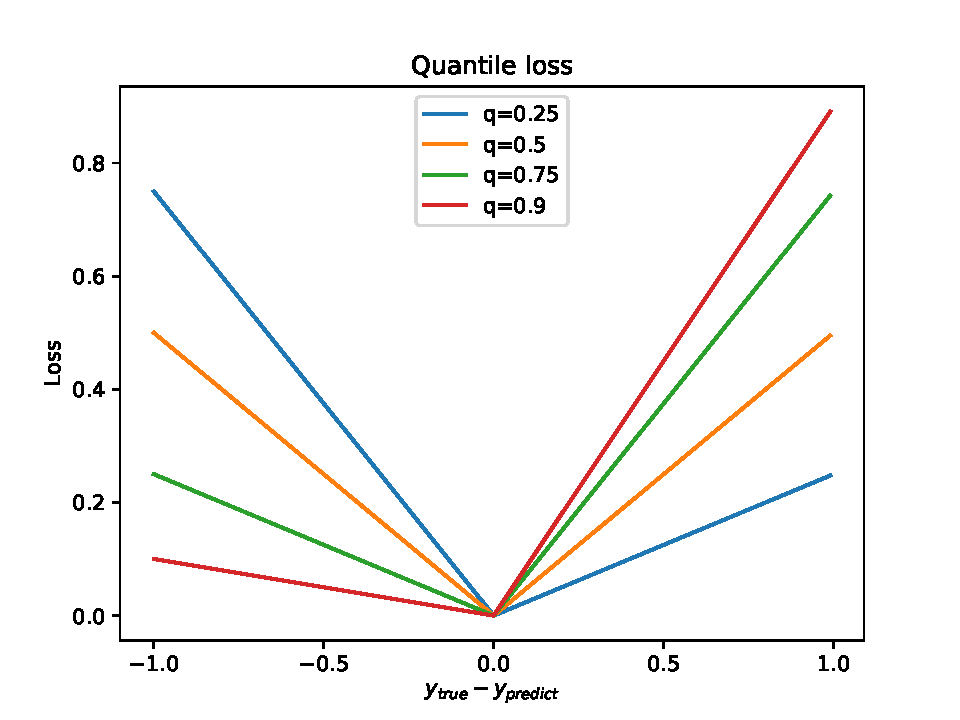
\includegraphics[width=0.8\textwidth]{images/quantile_loss.pdf}
    \caption{Quantile loss for different quantile values}
    \label{quantile_loss}
\end{figure}

Proposition 2 in \cite{Dabney2018} states that the combined quantile projection 
$\prod_{W_1}$ with the Bellman update $\mathcal{T}^\pi$ has a unique fixed point $\hat{Z}^\pi$, and the repeated application
of this operator, or its stochastic approximation, converges to $\hat{Z}^\pi$.

\subsection{Quantile Regression Temporal Difference Learning}
Temporal difference learning updates the estimated value function with a single unbiased 
sample following policy $\pi$.
Quantile regression allows to improve the estimate of the quantile function for some target
distribution Y(x), by observing samples $y\sim Y(x)$ and minimizing equation \eqref{eq:quantile_loss}.
Using the quantile regression loss, we can obtain an approximation with minimal 1-Wasserstein distance
from the original.
We can combine this with the distributional Bellman operator to give a target distribution
for quantile regression, creating the quantile regression temporal difference learning algorithm:

\begin{eqnarray}
    u=r+\gamma z' - \theta_i(x)\\
    \theta_i(x) \la \theta_i(x) + \alpha (\hat\tau_i - \delta_{u<0})\\
    a \backsim \pi(\cdot |x) , r \backsim R(x,a), x'\backsim P(\cdot |x,a), z' \backsim Z_\theta(x')
\end{eqnarray}

where $Z_\theta$ is a quantile distribution as in \eqref{eq:discrete_pdf} and $\theta_i(x)$ 
is the estimated value of $F_{Z^\pi(x)}^{-1}(\hat\tau_i)$ in state x.
